\documentclass[conference]{IEEEtran}
\usepackage[utf8]{inputenc}
\usepackage{graphicx}
\usepackage[main=english,portuguese]{babel}

\usepackage{color,soul} % TEMPORARIO => SÓ PARA VISUALIZAR TEXTO PENDENTE

\ifCLASSINFOpdf
\else
\fi
\hyphenation{op-tical net-works semi-conduc-tor}


\begin{document}

\title{Sistemas de visualização de\\redes metabólicas}

\author{\IEEEauthorblockN{Gabriella de O. Esteves}
\IEEEauthorblockA{Universidade de Brasília\\
Departamento de Ciência da Computação\\
Brasília, Brasil\\
Email: gabepk.ape@gmail.com}}


\maketitle

% As a general rule, do not put math, special symbols or citations
% in the abstract
\begin{abstract}
The abstract goes here.
\end{abstract}

% no keywords

\section{Introducão}

O metabolismo é isso X, ocorre por isso (síntese e degradação) e funciona com isso (moléculas, metabólitos).

Como o metabolismo tem sido representado computacionalmente (redes metabólicas)? Como as redes metabólicas tem sido visualizadas (estado da arte)? \\
Problema, objetivo. \\
Descrição dos capítulos.


\section{Redes Metabólicas}

\hl{Paragrafo intro} \\. As reações bioquímicas são alterações químicas que fornecem um ou mais produtos a partir de um ou mais substratos. Uma via metabólica é uma sequência de reações bioquímicas, cujo produto e subtrato são denominados de metabólitos, que podem ser catalisados por enzimas, as quais muitas vezes necessitam de compostos químicos chamados de co-fatores para realizarem suas atividades na célula. O conjunto de vias metabólicas de um organismo é chamado de rede metabólica. Todos estes elementos que compõem as redes metabólicas são dados biológicos estudados na área metabolômica. Nesta seção são apresentados três bancos de dados de redes metabólicas: KEGG\footnote{site kegg}, BIoCyc e Reactome.

LIVRO LEHNINGER

\subsection{Conceitos de Biologia Molecular}

O DNA é um conjunto de biomoléculas em um organismo que armazena informações, chamados de genes, referentes ao funcionamento de todas as suas células. Ele constitui o genoma em todos os seres vivos, com excessão dos vírus. A expressão dos genes é o processo no qual os genes são filtrados e utilizados na síntese de um produto, geralmente proteína. O método é segmentado em três etapas: transcrição (síntese de RNA mensageiro, mRNA, a partir de DNA), \textit{splicing} (filtragem do gene síntetizador de proteínas desejadas do mRNA) e tradução (síntese de proteína a partir do mRNA filtrado). Completo este processo, as proteínas resultantes poderão formar uma configuração tridimensional de até quatro níveis. As enzimas, por exemplo, são proteínas que podem ter estrutura terciária ou quaternária. \\
\indent \hl{Intro sobre sequenciamento de genoma} \\

\subsection{Conceitos de Metabolismo}

O papel das enzimas no metabolismo é realizar biosíntese/degradação de moléculas para produção de energia (catalisar) com o propósito de acelerar reações bioquímicas. Aquelas que possuem a mesma atividade enzimática porém estruturas físicas diferentes são chamadas isoenzimas. \hl{Ligar paragrafos}.  \\
\indent Quando o metabolismo exerce uma função fundamental no organismo, ele é classificado como metabolismo primário. Mitose e meiose são exemplos de metabolismos primários. Já quando o metabolismo não está relacionado a reprodução, desenvolvimento ou crescimento, ele não é essencial no organismo e, portanto, secundário. Os metabólitos secundários, apesar da aparente insignificância, podem ser antibióticos, por exemplo, e deste modo são bastante aplicados na medicina e na indústria \cite{waldeyr}.

\subsection{Banco de Dados de redes metabólicas}


\hl{Paragrafo intro}  \\. O KEGG (\textit{Kyoto Encyclopedia of Genes and Genomes}) é uma base de informações sobre sistemas biológicos em nível molecular, sobretudo sobre conjuntos de dados em larga escala gerados por sequenciamento de genoma \cite{keggOverview}. As informações sobre os sistemas podem ser dadas em forma de módulos, unidades funcionais com identificação otimizada para análise dos dados, em forma de \textit{brite}, coleção de arquivos estruturados hierarquicamente sobre as funções das entidades biológicos, ou em forma de vias, mapa de interações moleculares e reações químicas. Dado que o metabolismo é um conjunto de reações e transformações químicas, a maneira natural de representá-lo é por meio de uma rede de interações, ou seja, em forma de vias. O KEGG oferece uma ferramenta de busca de vias metabólicas sobre várias rede metabólica, dos vários organismos que constituem o banco de dados. É possível acessar o KEGG pela \textit{web} através do site \textit{http:\/\/www.kegg.jp\/}. \hl{Ligar paragrafos}.\\
\indent O BioCyc é um sistema de coleção de aproximadamente 7 mil bancos de dados chamados PGDBs (\textit{Pathway/Genome Databases}) pois possuem duas maneiras diferentes de representar as informações: modelo de vias metabólicas, que enfatiza as sequências de reações, substratos e produtos de múltiplos organismos, ou modelo de sequência genômica, que destaca a localização e descrição dos genes de cada organismo específico \cite{biocycIntro}. Os bancos PGDBs são organizado em três camadas de acordo com a frequência de atualizações/refinações e da maneira com que os dados foram obtidos. O BioCyc possui um banco de dados específico para redes metabólicas determinadas experimentalmente, chamado MetaCyc. Este é o único banco de dados multi-organismos do grupo BioCyc e ele é referência na ferramenta gratuita \textit{Pathway Tools} desenvolvida pelo instituto de pesquisa \textit{SRI International}.\hl{Ligar paragrafos} \\
\indent Reactoma é um banco de dados de reações de mudança de estado, ou seja, além de reações bioquímica, ele também abrange reações de ativação, de degradação e de ligação, por exemplo \cite{reactomeUsersguide}. Ele faz uma ligação sistemática entre as proteínas de um certo organismo e as funções moleculares do mesmo, fornecendo uma base de funções que pode ser utilizada para pesquisas sobre expressão de genes ou mutações somáticas. O Reactome disponibiliza o \textit{Pathway Browser}, uma rede geral para cada organismo, que representa os vários seus sistemas, como reprodução e metabolismo, por exemplo. Algumas sub-redes estão conectadas (por exemplo, replicação de DNA e ciclo de célula), outra não (por exemplo, contração muscular e reprodução). Nesta rede, cada nó representa uma via cujo número de entidade se reflete no raio do nó, e cada aresta representa a relação entre estas vias. O site ainda possui uma ferramenta de análise de dados baseada nas correspondências entre as reações na redes dos organismos comparados. \\
\hl{Frase final} \\

\section{Ferramentas de visualização de redes metabólicas}

\hl{Paragrafo inicial}

\subsection{KEGG Pathway Maps}

O KEGG oferece uma visao geral e uma visualização específica para análise de redes metabólicas. Na primeira, o grafo interativo apresenta uma perspectiva global das entidades do banco de dados do KEGG, chamadas de objetos KEGG. Neste panorama, a rede metabólica selecionada é destacada e é acompanhada de interações externas, que não possuem ligação direta com a rede análisada. Os nós representam compostos químicos e as arestas podem representar enzimas, reações e/ou \hl{otholog}. Na página do Atlas, a visualização das arestas pode ser filtrada, bem como as vias, de acordo com suas funções. A Figura \ref{terpenoid_meva_kegg} apresenta uma parte da via de biosíntese de terpenóide, que tem início no composto Acetyl-CoA, destacada sobre as demais. A outra maneira de visualizar esta via é acessando o objeto KEGG do tipo \textit{map} o qual ela representa (\textit{KEGG Pathway Map}). O mapa de vias é um diagrama de interações/reações moleculares entre enzimas desenhado manualmente. A via da Figura \ref{terpenoid_meva_kegg_solo} apresenta a mesma via da Figura \ref{terpenoid_meva_kegg}. \\

\begin{figure}[!t]
\centering
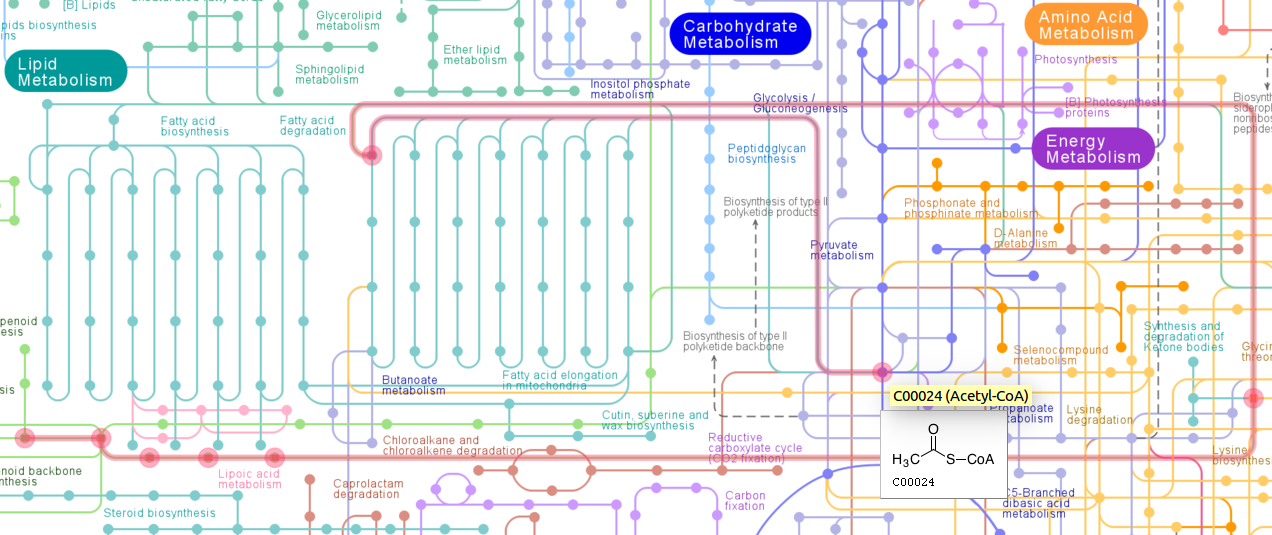
\includegraphics[width=0.5\textwidth]{terpenoid_meva_kegg.png}
\caption{KEGG}
\label{terpenoid_meva_kegg}
\end{figure}

\begin{figure}[!t]
\centering
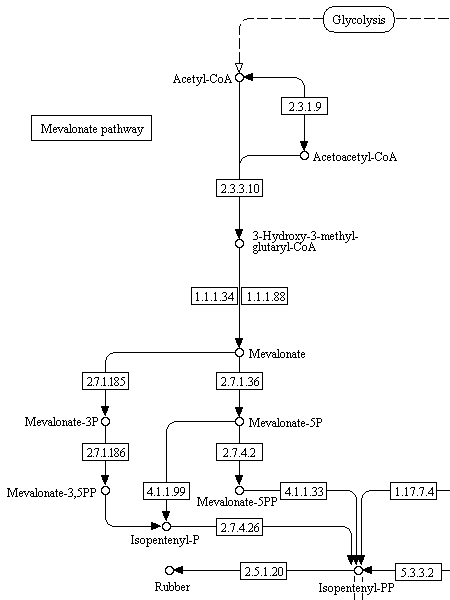
\includegraphics[width=0.4\textwidth]{terpenoid_meva_kegg_solo.png}
\caption{KEGG}
\label{terpenoid_meva_kegg_solo}
\end{figure}

\subsection{MetaCyc Pathway Tools}

O intituto SRI International oferece a ferramenta \textit{Pathway Tools} para busca, visualização e edição de dados do MetaCyc \cite{articleMetacyc}. Ela possui três componentes de análise:
\begin{itemize}
\item[1]\textbf{Pathologic}: Um PGDB é gerado a partir do genoma de um organismo e de vias metabólicas produziadas por um software de predição de vias; 
\item[2]\textbf{Pathway/Genome Editor}: Permite que curadores (especialistas responsáveis por verificar na literatura a corretude dos dados) possam refinar manualmente um PGDB, bem como importar ou exportar entidades de um PGDB para outro;
\item[3]\textbf{Pathway/Genome Navigator}: Oferece mecanismos de busca, visualização e anpalise de redes metabólicas.
\end{itemize}
\indent Além dessas funcionalidades principais, o Pathway Tools dispõe também de meios para geração de posters de genomas e mapas metabólicos a partir de PGDB, comparação de mapas metabólicos inteiros e exportação de PGDB em vários formatos \cite{MetacycDesktopVsWeb}. Via web, o MetaCyc oferece mecanismos básicos de análise metabolômica, tais como coloração de nós sobre redes (ou colagens de redes) metabólicas para geração de diagramas customizados e análise de níveis de metabólitos, por exemplo \cite{MetacycOmicAnalysis}.

\begin{figure}[!t]
\centering
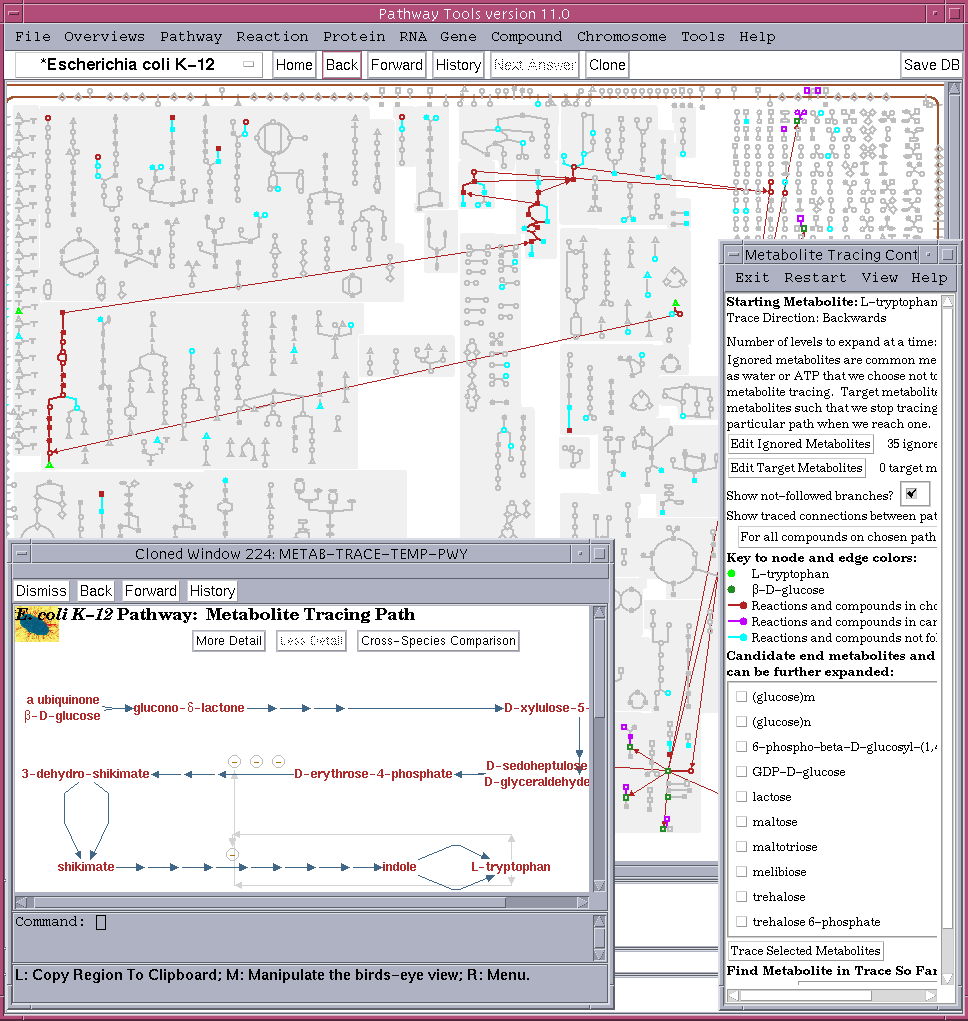
\includegraphics[width=0.4\textwidth]{biocyc-pathwaytool-desktop.png}
\caption{BioCyc}
\label{metacyc_arvore}
\end{figure}


\begin{figure}[!t]
\centering
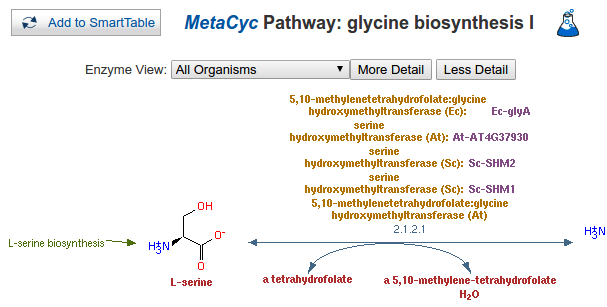
\includegraphics[width=0.5\textwidth]{metacyc_glycin_small.png}
\caption{BioCyc}
\label{metacyc_glycin_small}
\end{figure}

\subsection{Reactome}

\begin{figure}[!t]
\centering
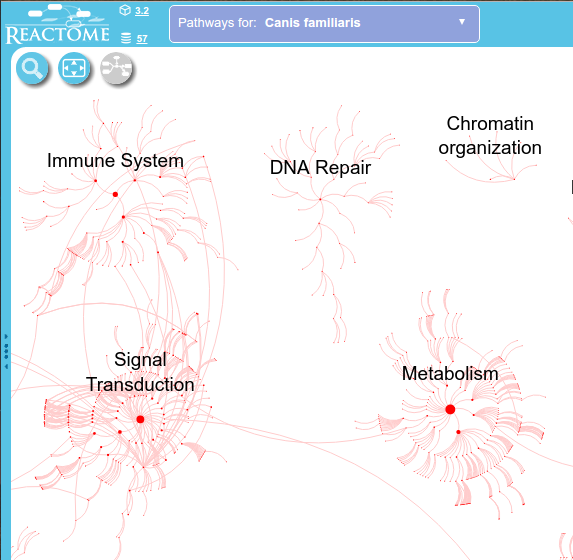
\includegraphics[width=0.5\textwidth]{reactome_canis_small.png}
\caption{Reactome}
\label{reactome_canis_small}
\end{figure}

\begin{itemize}
\item http:\/\/wiki.reactome.org\/index.php\/Usersguide
\item The Reactome pathway knowladgebase
\end{itemize}

\subsection{Cytoscape}

\begin{itemize}
\item http:\/\/www.cytoscape.org\/what\_is\_cytoscape.html
\item Cytoscape: A Software Environment for Integrated Models of Biomolecular Interaction Networks
\end{itemize}

\section{Conclusão}

Conclusão





% An example of a floating figure using the graphicx package.
% Note that \label must occur AFTER (or within) \caption.
% For figures, \caption should occur after the \includegraphics.
% Note that IEEEtran v1.7 and later has special internal code that
% is designed to preserve the operation of \label within \caption
% even when the captionsoff option is in effect. However, because
% of issues like this, it may be the safest practice to put all your
% \label just after \caption rather than within \caption{}.
%
% Reminder: the "draftcls" or "draftclsnofoot", not "draft", class
% option should be used if it is desired that the figures are to be
% displayed while in draft mode.
%
%\begin{figure}[!t]
%\centering
%\includegraphics[width=2.5in]{myfigure}
% where an .eps filename suffix will be assumed under latex, 
% and a .pdf suffix will be assumed for pdflatex; or what has been declared
% via \DeclareGraphicsExtensions.
%\caption{Simulation results for the network.}
%\label{fig_sim}
%\end{figure}

% Note that the IEEE typically puts floats only at the top, even when this
% results in a large percentage of a column being occupied by floats.


% An example of a double column floating figure using two subfigures.
% (The subfig.sty package must be loaded for this to work.)
% The subfigure \label commands are set within each subfloat command,
% and the \label for the overall figure must come after \caption.
% \hfil is used as a separator to get equal spacing.
% Watch out that the combined width of all the subfigures on a 
% line do not exceed the text width or a line break will occur.
%
%\begin{figure*}[!t]
%\centering
%\subfloat[Case I]{\includegraphics[width=2.5in]{box}%
%\label{fig_first_case}}
%\hfil
%\subfloat[Case II]{\includegraphics[width=2.5in]{box}%
%\label{fig_second_case}}
%\caption{Simulation results for the network.}
%\label{fig_sim}
%\end{figure*}
%
% Note that often IEEE papers with subfigures do not employ subfigure
% captions (using the optional argument to \subfloat[]), but instead will
% reference/describe all of them (a), (b), etc., within the main caption.
% Be aware that for subfig.sty to generate the (a), (b), etc., subfigure
% labels, the optional argument to \subfloat must be present. If a
% subcaption is not desired, just leave its contents blank,
% e.g., \subfloat[].


% An example of a floating table. Note that, for IEEE style tables, the
% \caption command should come BEFORE the table and, given that table
% captions serve much like titles, are usually capitalized except for words
% such as a, an, and, as, at, but, by, for, in, nor, of, on, or, the, to
% and up, which are usually not capitalized unless they are the first or
% last word of the caption. Table text will default to \footnotesize as
% the IEEE normally uses this smaller font for tables.
% The \label must come after \caption as always.
%
%\begin{table}[!t]
%% increase table row spacing, adjust to taste
%\renewcommand{\arraystretch}{1.3}
% if using array.sty, it might be a good idea to tweak the value of
% \extrarowheight as needed to properly center the text within the cells
%\caption{An Example of a Table}
%\label{table_example}
%\centering
%% Some packages, such as MDW tools, offer better commands for making tables
%% than the plain LaTeX2e tabular which is used here.
%\begin{tabular}{|c||c|}
%\hline
%One & Two\\
%\hline
%Three & Four\\
%\hline
%\end{tabular}
%\end{table}


% Note that the IEEE does not put floats in the very first column
% - or typically anywhere on the first page for that matter. Also,
% in-text middle ("here") positioning is typically not used, but it
% is allowed and encouraged for Computer Society conferences (but
% not Computer Society journals). Most IEEE journals/conferences use
% top floats exclusively. 
% Note that, LaTeX2e, unlike IEEE journals/conferences, places
% footnotes above bottom floats. This can be corrected via the
% \fnbelowfloat command of the stfloats package.



% conference papers do not normally have an appendix


% use section* for acknowledgment
\section*{Agradecimento}


% trigger a \newpage just before the given reference
% number - used to balance the columns on the last page
% adjust value as needed - may need to be readjusted if
% the document is modified later
%\IEEEtriggeratref{8}
% The "triggered" command can be changed if desired:
%\IEEEtriggercmd{\enlargethispage{-5in}}

% references section
% manually copy in the resultant .bbl file
% set second argument of \begin to the number of references
% (used to reserve space for the reference number labels box)
\begin{thebibliography}{1}
  
\bibitem{waldeyr}
W.M.C.~Silva, \emph{Método para reconstrução in silico de redes metabólicas de fungos: um estudo de caso para o Paracoccidioides lutzii}. \hskip 1em plus 0.5em minus 0.4em\relax Universidade de Brasília, 2014.

\bibitem{keggOverview}
Kyoto Encyclopedia of Genes and Genome, \emph{KEGG Overview} \hskip 1em plus 0.5em minus 0.4em\relax \emph{http://www.kegg.jp/kegg/kegg1a.html} visitado em 01 de Outubro de 2016.

\bibitem{biocycIntro}
SRI International and BioCyc Database Collection, \emph{Introduction to BioCyc} \hskip 1em plus 0.5em minus 0.4em\relax \emph{http://biocyc.org/intro.shtml} visitado em 01 de Outubro de 2016.

\bibitem{reactomeUsersguide}
Reactome, a curated pathway database, \emph{Usersguide} \hskip 1em plus 0.5em minus 0.4em\relax \emph{http://wiki.reactome.org/index.php/Usersguide} visitado em 01 de Outubro de 2016.

\bibitem{articleMetacyc}
Caspi, Ron et al. \emph{MetaCyc: A Multiorganism Database of Metabolic Pathways and Enzymes.} \hskip 1em plus 0.5em minus 0.4em\relax Nucleic Acids Research 34.Database issue (2006): D511–D516. PMC. Web. 5 Oct. 2016.

\bibitem{MetacycDesktopVsWeb}
SRI International and BioCyc Database Collection, \emph{Comparison of Desktop and Web Modes of Pathway Tools} \hskip 1em plus 0.5em minus 0.4em\relax \emph{http://biocyc.org/desktop-vs-web-mode.shtml} visitado em 03 de Outubro de 2016.

\bibitem{MetacycOmicAnalysis}
SRI International and BioCyc Database Collection, \emph{Omics Data Analysis} \hskip 1em plus 0.5em minus 0.4em\relax \emph{http://metacyc.org/PToolsWebsiteHowto.shtml\#omicsDataAnalysis} visitado em 04 de Outubro de 2016.

\end{thebibliography}





\end{document}


